\chapter{Spatial Prediction of Air Quality}\label{prediction_evaluation}

	\section{Motivation}\label{prediction_evaluation_motivation}

		In sampling data it is almost inevitable that some information will be missed. In order to accurately reconstruct the original data we must take certain precautions. One of these precautions is making sure that we sample at a rate high enough to reconstruct all information. This rate goes by the term \emph{Nyquist rate}~\cite{nyquistrate}. The Nyquist rate is the rate of taking measurements such that the original information can be reconstructed without aliasing occurring. This essentially means that we need to have a sample rate of twice the rate of the smallest changes in a signal. If we do not have this sampling rate then it is possible for us to lose information during the sampling process such as that seen in figure~\ref{fig:nyquist_example}.

		\centerimagewideanywhere{./images/Nyquist_Example.png}{An example of a sample rate on the function $y = sin(4x)$ being insufficient. The reconstructed function from the sampled points is $y = -sin(1.235x)$, showing that the sample rate of 1.2 is insufficient for the graph since its period is $\frac{2\pi}{4} \equiv 1.570$. A sample rate of $\frac{1.570}{2} \equiv 0.785$ is required to be sufficient.}{fig:nyquist_example}

		When measuring air quality we almost certainly will not meet the Nyquist rate and therefore need to compensate. Without any interpolation or extrapolation methods the best we can do is generate data similar to that seen in figure~\ref{fig:stationarypollutantbuildup}. In this figure we see that we only have information where pollutants were measured. In this case it was done with a sensor on a bus and therefore limited to the roads. 

		\centerimageanywhere{0.6\textwidth}{./images/StationaryPollutantBuildUp.png}{A map of air pollution around Edinburgh city centre. This data was recorded and mapped during the first year of the project. The image uses \emph{Open Street Map}.}{fig:stationarypollutantbuildup}

		\centerimageanywhere{.5\textwidth}{./images/zurichpm.jpg}{A heatmap of particulate matter in Zurich. The higher pollution levels can clearly be seen to follow transport infrastructure. This image is from the OpenSense projects website~\cite{opensensezurich}.}{fig:zurichheatmap}

		The solution is to interpolate and extrapolate our data so that what we see in figure~\ref{fig:stationarypollutantbuildup} can be converted into something similar to figure~\ref{fig:zurichheatmap}, where we have estimations of pollutant levels in areas where we did not take measurements. 

		With air quality data, many institutes and organisations use complex methods of interpolating the data such as (LUR)~\cite{lurtraffic}. LUR and other advanced models~\cite{reviewofaqmodels} have advantages over simple interpolation models in that they can take information about the sampling environment into account. By providing this auxiliary information, such as known sources of pollution, terrain, buildings, etc. we can greatly improve the accuracy of the estimations that these advanced models produce, achieving results similar to that which would be generated should our sample rate match the Nyquist rate. These models are not without their disadvantages however. One of the main drawbacks of these is the considerably complexity of development and use. As such it would be useful to determine if simple interpolation algorithms, such as those designed for image or sound processing, are effective at interpolation air quality data sets. The algorithms which will be tested are those discussed in section~\ref{background_interpolation_methods}. These algorithms are: 

		\begin{itemize}
	        \item Nearest neighbour interpolation
			\item Inverse distance weighting interpolation
	        \item Natural neighbour interpolation
	        \item Bilinear interpolation
	        \item Bicubic interpolation
	        \item Barnes interpolation
	    \end{itemize}

	    The bilinear and bicubic algorithms are generally used for interpolating pixels in images when resized. Natural neighbour, nearest neighbour and inverse distance weighted are more generic interpolation algorithms, and Barnes interpolation has seen application in weather forecasting~\cite{barnesinterpolation}. These algorithms were chosen as all are commonly used and are simple to understand. 



	\section{Methodology}\label{prediction_evaluation_methodology}

		Our method of evaluation is simple. By applying the various interpolation algorithms to data sets, we will have predicted values at points where there are no measurements. By comparing these predicted values and the actual values recorded, either from other data sources or by removing select data points from the original data set, we will have a metric for comparing the efficiency of the various algorithms. 

		\subsection{Data Sets}\label{prediction_evaluation_methodology_data_sets}

			\subsubsection{Air Quality Scotland}\label{prediction_evaluation_methodology_data_sets_air_quality_scotland}

				The data set from \emph{Air Quality Scotland} consists of eight static air quality monitoring stations across Edinburgh. Out of these eight stations, five form the convex hull of the data set, and one of the internal stations is in a high traffic zone. The result of this is that we only have three points which we can use to check our calculations, and one of these will have a large discrepancy between the actual values and the estimated values due to the nature of interpolation. However, one advantage that this data set does provide is that there are three different chemical readings to use: $NO$, $NO_{2}$, and $NO_{X}$.

				This data set provides readings which are aggregated into one hour means. As such we do not have the issue of temporal slicing as discussed in the next section.

			\subsubsection{OpenSense}\label{prediction_evaluation_methodology_data_sets_opensense}

				This data set, provided by the \emph{OpenSense} group at \emph{ETH Zurich}, provides ozone concentrations based on measurements taken from trams moving around the city of Zurich, Switzerland. This data set only has measurements along the tram tracks, similar to how data would be provided along bus routes with a physical implementation of this system. 

				\centerimageanywhere{0.7\textwidth}{./images/Zurich_Ozone.png}{A scatter plot of the Zurich data points. The hue of the colour of the points is directly proportional to the Ozone concentration.}{fig:zurich_ozone}

				This data set is the most realistic in terms of mimicking the data from buses around Edinburgh, however it does pose certain problems. The foremost of these is that there are only two static sensors which we can use to determine the accuracy of our algorithms. The fewer static sensors we have to use for results validation, the less certainty we will have the in the accuracy of results.

				A second problem, is one which affects most data sets which we would use. That is the issues caused by the temporal changes in the data. If we were to take the measurements at any given point in time we would only have as many data points as there are sensors, which may not provide sufficient coverage. We can assume that pollutant levels do not change so quickly in that we would have extreme differences between readings over short time frames. By making this assumption we can select a temporal window of measurements and so can increase the number of readings we have. These readings will also be at different locations due to the motion of the trams, giving a better representation of the actual data, and thereby improving the accuracy of our algorithms. 

				In taking this temporal window we risk missing out on some information. Should a pollutant change rapidly in the space of a single window, this information would be lost, and may indeed skew the results. 

				Unfortunately this data set arrived late in the project and as such was not available for the initial round of evaluation and writing of this report. The findings from this data set are shown in a sub-section at the end of the results section, numbered~\ref{prediction_evaluation_results_opensense_data_set}.

		\subsection{Data Structure}\label{prediction_evaluation_methodology_data_structure}
			
			In order to use these data sets in the various algorithms we must change the data structure slightly. Two of the algorithms, bilinear interpolation, and bilinear interpolation, \emph{only} work when the data is on a regular grid, which these data sets are not. As such we need to map them onto a regular grid. For the algorithms which are not limited to a grid we do not have to

			With the Zurich data set the area which we are taking measurements from is roughly $5km$ by $5km$. By setting a resolution of 200 by 200 for the grid we can calculate the interpolated values in regions roughly $25m$ by $25m$. Using the same resolution on the Edinburgh data we move our data points from a map of size $15km$ by $9km$ to a grid with cells of size $75m$ by $45m$. 


    \section{Results}\label{prediction_evaluation_results}

        \subsection{Nearest Neighbour}\label{prediction_evaluation_results_nearest_neighbour}

	        \centerimage{0.7\textwidth}{./images/Nearest_Neighbour_Zurich.png}{The result of applying the nearest neighbour algorithm to the data seen in figure~\ref{fig:zurich_ozone}.}{fig:nearest_neighbour_zurich}

	        The nearest neighbour algorithm is our simplest interpolation method, and due to that it acts as a baseline to compare to. We would expect this algorithm to have the worst performance on most data sets. When we apply the nearest neighbour algorithm to the data set seen in figure~\ref{fig:zurich_ozone} we get a result similar to that seen in figure~\ref{fig:nearest_neighbour_zurich}. When we apply it to the Edinburgh data set we get results seen in figure~\ref{fig:nearest_neighbour_difference_results}. 

			\centerimageanywhere{0.8\textwidth}{./images/Nearest_Neighbour_Percentage_Differences.png}{The results of running the nearest neighbour algorithm as a scatter plot, averaged across three different measurement points.}{fig:nearest_neighbour_difference_results}

			From this scatter plot we get the first information about our interpolation algorithm. Initially we can see that $NO_{2}$ has a much lower percentage difference on average than the other pollutants. We can also see that there seems to be some correlation between the percentage difference of the value of $NO$ and the value of $NO_{X}$. 

			In order to have a metric which allows us to evaluate the performance we must take the mean across all time periods. This data is shown in table~\ref{tab:nearest_neighbour_difference_results_mean}. 

			\begin{table}
				\centering
	    		\begin{tabular}{|c|c|}
	    			\hline
			        Pollutant & Difference (\%) \\ \hline
					$NO$ & 23.87 \\
					$NO_{2}$ & 3.75 \\
					$NO_{X}$ & 13.49 \\ \hline
				\end{tabular}
				\caption{The mean results of the data in figure~\ref{fig:nearest_neighbour_difference_results}.}
				\label{tab:nearest_neighbour_difference_results_mean}
			\end{table}

		\subsection{Nearest Neighbour}\label{prediction_evaluation_results_nearest_neighbour_convolution_filter}

			\centerimage{0.7\textwidth}{./images/Nearest_Neighbour_Sigma_6_Zurich.png}{The result of applying the nearest neighbour with convolution filter algorithm to the data seen in figure~\ref{fig:zurich_ozone}. This is the result of setting $\sigma$ to the value of $2^{6}$.}{fig:nearest_neighbour_blur_zurich}

			As was mentioned in section~\ref{background_interpolation_methods_nearest_neighbour}, a possible optimisation to the nearest neighbour algorithm is to apply a convolution filter to it. In this case we will use a Gaussian blur as our convolution filter, and henceforth the algorithm will be known as ``blurry neighbour''. The formula for applying a Gaussian blur in two dimensions~\cite{gaussianblur} is:

			\begin{align*}
				G(x,y) = \frac{1}{2\pi\sigma^{2}} e^{-\frac{x^{2} + y^{2}}{2\sigma^{2}}}
			\end{align*}

			As we can see from this equation, we have introduced a new parameter, $\sigma$. In order to evaluate the effectiveness of this algorithm we must also have an optimal value of $\sigma$. To find this optimal value, the tests were run the same way as they were in the previous section, but this time we also had $\sigma$ as a variable. By taking the mean of the results across all time frames and plotting this against the value of $\sigma$, our results are that of figure~\ref{fig:nearest_neighbour_convolution_sigma_results}. 

			\iffalse
				\begin{table}
					\centering
		    		\begin{tabular}{|c|c|c|c|c|c|c|}
		    			\hline
						Pollutant & Sigma & Difference \\ \hline
						$NO$ & 1 & 202.40 \\
						$NO$ & 2 & 200.90 \\
						$NO$ & 4 & 189.34 \\
						$NO$ & 8 & 182.73 \\
						$NO$ & 16 & 189.79 \\
						$NO$ & 32 & 187.60 \\
						$NO$ & 64 & 174.09 \\
						$NO$ & 128 & 166.21 \\
						$NO$ & 256 & 163.23 \\
						$NO$ & 512 & 163.22 \\
						$NO_{2}$ & 1 & 167.43 \\
						$NO_{2}$ & 2 & 166.80 \\
						$NO_{2}$ & 4 & 157.71 \\
						$NO_{2}$ & 8 & 147.90 \\
						$NO_{2}$ & 16 & 145.19 \\
						$NO_{2}$ & 32 & 144.66 \\
						$NO_{2}$ & 64 & 133.29 \\
						$NO_{2}$ & 128 & 127.46 \\
						$NO_{2}$ & 256 & 126.20 \\
						$NO_{2}$ & 512 & 126.20 \\
						$NO_{x}$ & 1 & 166.89 \\
						$NO_{x}$ & 2 & 166.13 \\
						$NO_{x}$ & 4 & 156.69 \\
						$NO_{x}$ & 8 & 146.44 \\
						$NO_{x}$ & 16 & 143.22 \\
						$NO_{x}$ & 32 & 142.87 \\
						$NO_{x}$ & 64 & 132.21 \\
						$NO_{x}$ & 128 & 126.95 \\
						$NO_{x}$ & 256 & 125.87 \\
						$NO_{x}$ & 512 & 125.87 \\ \hline
					\end{tabular}
					\caption{The mean results of varying the value of $\sigma$ in applying a Gaussian blur to the nearest neighbour results.}
					\label{tab:nearest_neighbour_convolution_sigma_results}
				\end{table}
			\fi

			\centerimageanywhere{0.7\textwidth}{./images/Nearest_Neighbour_Gaussian_Blur.png}{The mean results of varying the value of $\sigma$ in applying a Gaussian blur to the nearest neighbour results.}{fig:nearest_neighbour_convolution_sigma_results}

			This data shows a clear downward trend of the data, which appears to level out where sigma has a value somewhere between 128 and 512. As such, a suggested value of $\sigma$ would be 256. 

			After finding this optimal value of sigma, the tests from section~\ref{prediction_evaluation_results_nearest_neighbour} will be run once again, but with the Gaussian blur applied with $\sigma$ having the value 256. The results of this test are as follows:

			\centerimageanywhere{0.7\textwidth}{./images/Nearest_Neighbour_256.png}{The mean results of the different pollutants across time frames when a Gaussian blur is applied to the nearest neighbour results, with a value of $\sigma$ equal to 256.}{fig:nearest_neighbour_256}

			Taking the mean of the absolute value across all time frames and locations we get the results in table~\ref{tab:nearest_neighbour_convolution_results}.

			\begin{table}
				\centering
	    		\begin{tabular}{|c|c|}
	    			\hline
					Pollutant & Difference (\%) \\ \hline
					$NO$ & 24.52 \\
					$NO_{2}$ & 13.05 \\
					$NO_{X}$ & 18.99 \\
					\hline 
				\end{tabular}
				\caption{The mean results of the nearest neighbour algorithm when applying a Gaussian blur with $\sigma$ equal to 256.}
				\label{tab:nearest_neighbour_convolution_results}
			\end{table}

			Comparing this table, \ref{tab:nearest_neighbour_convolution_results}, to the non-Gaussian blur results in table~\ref{tab:nearest_neighbour_difference_results_mean}, we can see that Gaussian blurring has in fact lowered the accuracy of our interpolation methods, despite us being in control of the blur radius and can tune it to our data set. 

        \subsection{Inverse Distance Weighting}\label{prediction_evaluation_results_inverse_distance_weighting}

        	\centerimage{0.7\textwidth}{./images/IDW_Zurich.png}{The result of applying the inverse distance weighting algorithm to the data seen in figure~\ref{fig:zurich_ozone}. This is the result of setting the power parameter to 10.}{fig:idw_zurich}

        	Similarly to blurry neighbour, we have an extra parameter with inverse distance weighting (IDW). This parameter is the power parameter. Due to the fact that as the power parameter approaches infinity, the algorithm approaches nearest neighbour, we expect to see an improvement over nearest neighbour for lower values of p, based on our estimate of nearest neighbour being the worst performing algorithm.

        	Running the same tests as before, with IDW and a variable power parameter the results are seen in figure~\ref{fig:idw_power_all}.

        	\centerimageanywhere{0.6\textwidth}{./images/IDW_P_All.png}{The mean of all pollutants across all times across all locations, with a varying power parameter, which is also known as the distance factor.}{fig:idw_power_all}

        	We can clearly see from this graph that there is a minima with a power rating of around 3. As such we can take 3 to be the optimal and run the tests again. The results of this are shown in table~\ref{tab:idw_results}.

        	\begin{table}
				\centering
	    		\begin{tabular}{|c|c|}
	    			\hline
					Pollutant & Mean Difference (\%) \\ \hline
					$NO$ & 145.18 \\
					$NO_{2}$ & 17.54 \\
					$NO_{X}$ & 55.45 \\
					\hline
				\end{tabular}
				\caption{The mean results of IDW with power parameter equal to 256}
				\label{tab:idw_results}
			\end{table}

			When we compare these results to that of the simpler nearest neighbour algorithm we see that this algorithm is also much worse. As with the result in section~\ref{prediction_evaluation_results_nearest_neighbour_convolution_filter} it is likely that this is due to a lack of data points in the Edinburgh data set.

			One further thing which we must pay attention to, particularly in this algorithm, is the varying parameters for different pollutants. Figure~\ref{fig:idw_power_all} shows the mean of all pollutants across all times and locations. If we separate the pollutants then we get very different charts as seen in figure~\ref{fig:idw_pollutant_compare}.

			\begin{figure}
                \centering
                \begin{subfigure}{0.5\textwidth}
                    \centering
                    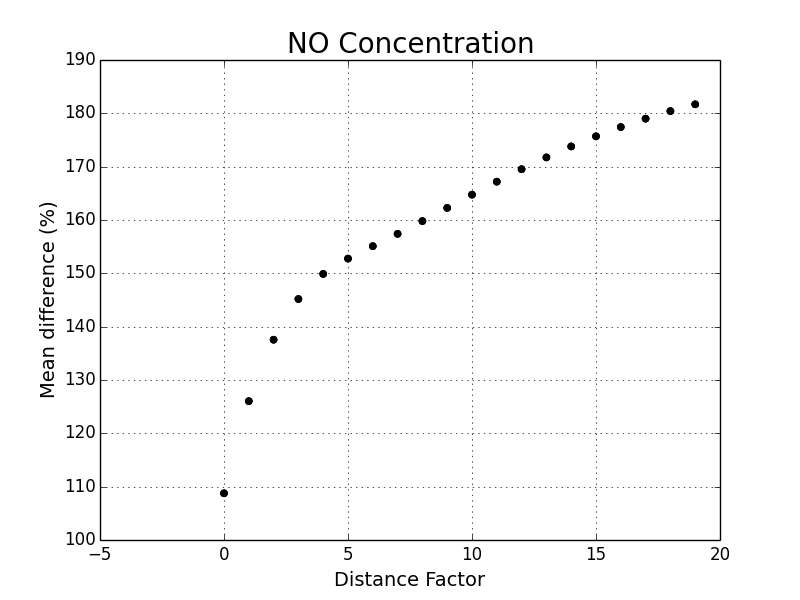
\includegraphics[width=\linewidth]{./images/IDW_P_NO.png}
                    \caption{}
                    \label{fig:idw_power_NO}
                \end{subfigure}%
                \begin{subfigure}{0.5\textwidth}
                    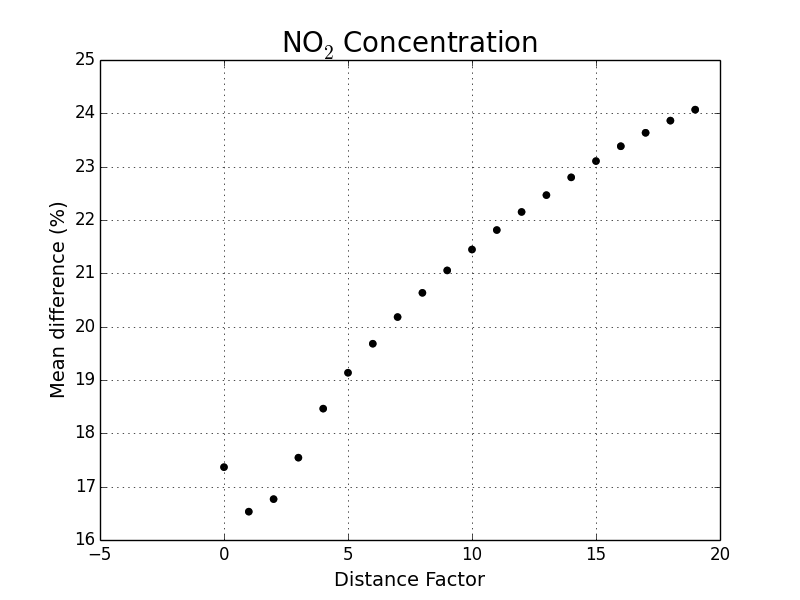
\includegraphics[width=\linewidth]{./images/IDW_P_NO2.png}
                    \caption{}
                    \label{fig:idw_power_NO2}
                \end{subfigure}
                \begin{subfigure}{0.5\textwidth}
                    \centering
                    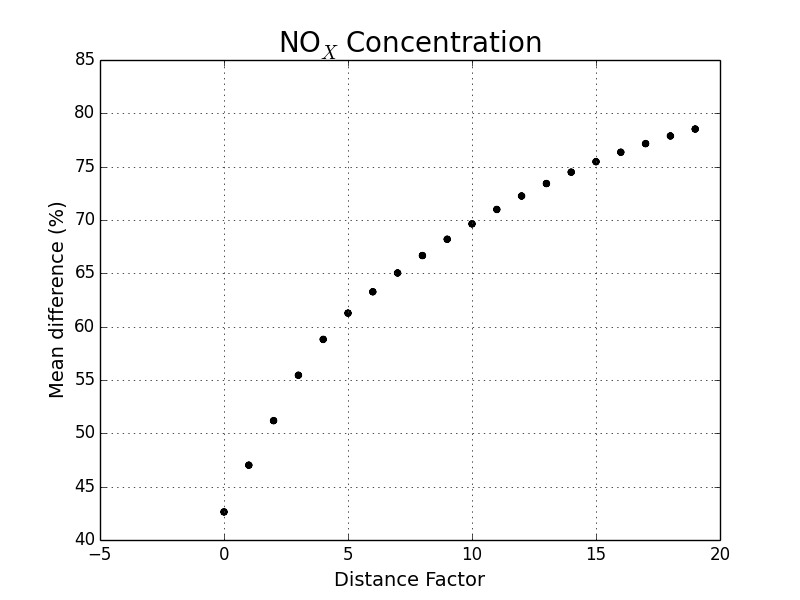
\includegraphics[width=\linewidth]{./images/IDW_P_NOx.png}
                    \caption{}
                    \label{fig:idw_power_NOx}
                \end{subfigure}
                \caption{These figures show how the optimal power parameter varies depending on the pollutant being measured.}
                \label{fig:idw_pollutant_compare}
            \end{figure}

            The minima seen in figure~\ref{fig:idw_power_all} is missing in two out of the three charts here. As such, the $NO_{2}$ reading is clearly dominating the others in the mean chart. From this it is clear that, at least for IDW, we must pay attention to all pollutants separately when testing with variable algorithm parameters. 

            If we run the tests once more, this time keeping pollutants separate, a very different picture is presented, seen in table~\ref{tab:idw_results_2}.

			\begin{table}
				\centering
	    		\begin{tabular}{|c|c|c|}
	    			\hline
					Pollutant & Combined Mean Difference (\%) & Mean Difference (\%) \\ \hline
					$NO$ & 145.18 & 24.98 \\
					$NO_{2}$ & 17.54 & 7.59 \\
					$NO_{X}$ & 55.45 & 18.98 \\
					\hline
				\end{tabular}
				\caption{The mean results of IDW with the optimal power parameter for each pollutant.}
				\label{tab:idw_results_2}
			\end{table} 

			From table~\ref{tab:idw_results_2} we can see that having a power parameter specified for each pollutant is an extreme improvement on the overall performance of the algorithm. 

		\subsection{Natural Neighbour}\label{prediction_evaluation_results_natural_neighbour}

        	\centerimage{0.7\textwidth}{./images/Natural_Neighbour_Zurich.png}{The result of applying the natural neighbour algorithm to the data seen in figure~\ref{fig:zurich_ozone}.}{fig:natural_neighbour_zurich}

        	With the natural neighbour interpolation algorithm, we have no optional parameters and the results are much simpler to calculate. We run the same tests as with IDW and average across all locations and time frames to get the results shown in table~\ref{tab:natural_neighbour_results}.

        	\begin{table}
				\centering
	    		\begin{tabular}{|c|c|}
	    			\hline
					Pollutant & Mean Difference (\%) \\ \hline
					$NO$ & 25.37 \\
					$NO_{2}$ & 5.89 \\
					$NO_{X}$ & 16.84 \\
					\hline
				\end{tabular}
				\caption{The mean results of natural neighbour interpolation.}
				\label{tab:natural_neighbour_results}
			\end{table} 

        \subsection{Bilinear}\label{prediction_evaluation_results_bilinear}

        	\centerimage{0.7\textwidth}{./images/Bilinear_Zurich.png}{The result of applying the bilinear algorithm to the data seen in figure~\ref{fig:zurich_ozone}.}{fig:bilinear_zurich}

        	Again, we have no optional parameters in the bilinear interpolation algorithm and so the same methods are previously are applied and shown in table~\ref{tab:bilinear_results}.

        	\begin{table}
				\centering
	    		\begin{tabular}{|c|c|}
	    			\hline
					Pollutant & Mean Difference (\%) \\ \hline
					$NO$ & 29.37 \\
					$NO_{2}$ & 5.08 \\
					$NO_{X}$ & 18.62 \\
					\hline
				\end{tabular}
				\caption{The mean results of bilinear interpolation.}
				\label{tab:bilinear_results}
			\end{table} 

        \subsection{Bicubic}\label{prediction_evaluation_results_bicubic}

        	\centerimage{0.7\textwidth}{./images/Bicubic_Zurich.png}{The result of applying the bicubic algorithm to the data seen in figure~\ref{fig:zurich_ozone}.}{fig:bicubic_zurich}

			The bicubic algorithm is similar to the bilinear algorithm and we once again use the same methods as before. The results are shown in table~\ref{tab:bicubic_results}.

        	\begin{table}
				\centering
	    		\begin{tabular}{|c|c|}
	    			\hline
					Pollutant & Mean Difference (\%) \\ \hline
					$NO$ & 18.38 \\
					$NO_{2}$ & 4.10 \\
					$NO_{X}$ & 11.22 \\
					\hline
				\end{tabular}
				\caption{The mean results of bicubic interpolation.}
				\label{tab:bicubic_results}
			\end{table} 

        \subsection{Barnes}\label{prediction_evaluation_results_barnes}

        	\centerimage{0.7\textwidth}{./images/Barnes_Zurich.png}{The result of applying the nearest neighbour algorithm to the data seen in figure~\ref{fig:zurich_ozone}. This is the result of a single pass with a distance parameter of $2^{15}$.}{fig:barnes_zurich}

        	Similarly to the blurry neighbour algorithm and IDW, Barnes interpolation has parameters which need to be tuned in order to get the best performance. These parameters are the number of error correcting passes we make over the data, and the distance constant which we use to weight the values we use to interpolate. As we have seen in previously, we should measure the result for each pollutant separately in order to achieve the best results. 

        	As discussed in section~\ref{background_interpolation_methods_barnes}, the greater the number of error correcting passes, the more the result converges to a single value, which can be seen occurring in figure~\ref{fig:barnes_distance_factor_results_NO}. In the interest of calculation time the number of passes has been limited to 24. 

        	As we can see, with no error correcting passes, we have a reasonable approximation of the result. Subsequent passes correct the error more and more. In order to determine the changes for different distance factors a test was run with the distance factor changing. The results of this test can be seen in figure~\ref{fig:barnes_distance_factor_results_NO}.

        	\centerimagewideanywhere{./images/Barnes_Distance_Factor_NO.png}{A scatter plot showing the error field difference for the ten different distance factors with the $NO$ pollutant.}{fig:barnes_distance_factor_results_NO}

        	From this graph it is clear that the greater the distance factor, the greater the difference successive passes make. This appears to continue until a distance of around $2^{17}$, which is also result with the lowest difference. At this point the difference made by applying many passes begins to decrease again. Furthermore we can see that the difference between passes decreases as the number of passes increases. As mentioned previously, due to computational time requirements these results were only calculated to 24 passes. However, increasing the runtime by 5 more passes, a run time increase of 20\%, would only yield a potential accuracy increase of around a one hundredth of one percent. 

        	When we apply the same analysis to the pollutants $NO_{2}$ and $NO_{X}$, we get the results seen in figure~\ref{fig:barnes_distance_factor_results_NO2_NOx}. 

        	\begin{figure}
                \centering
                \begin{subfigure}{\textwidth}
                    \centering
                    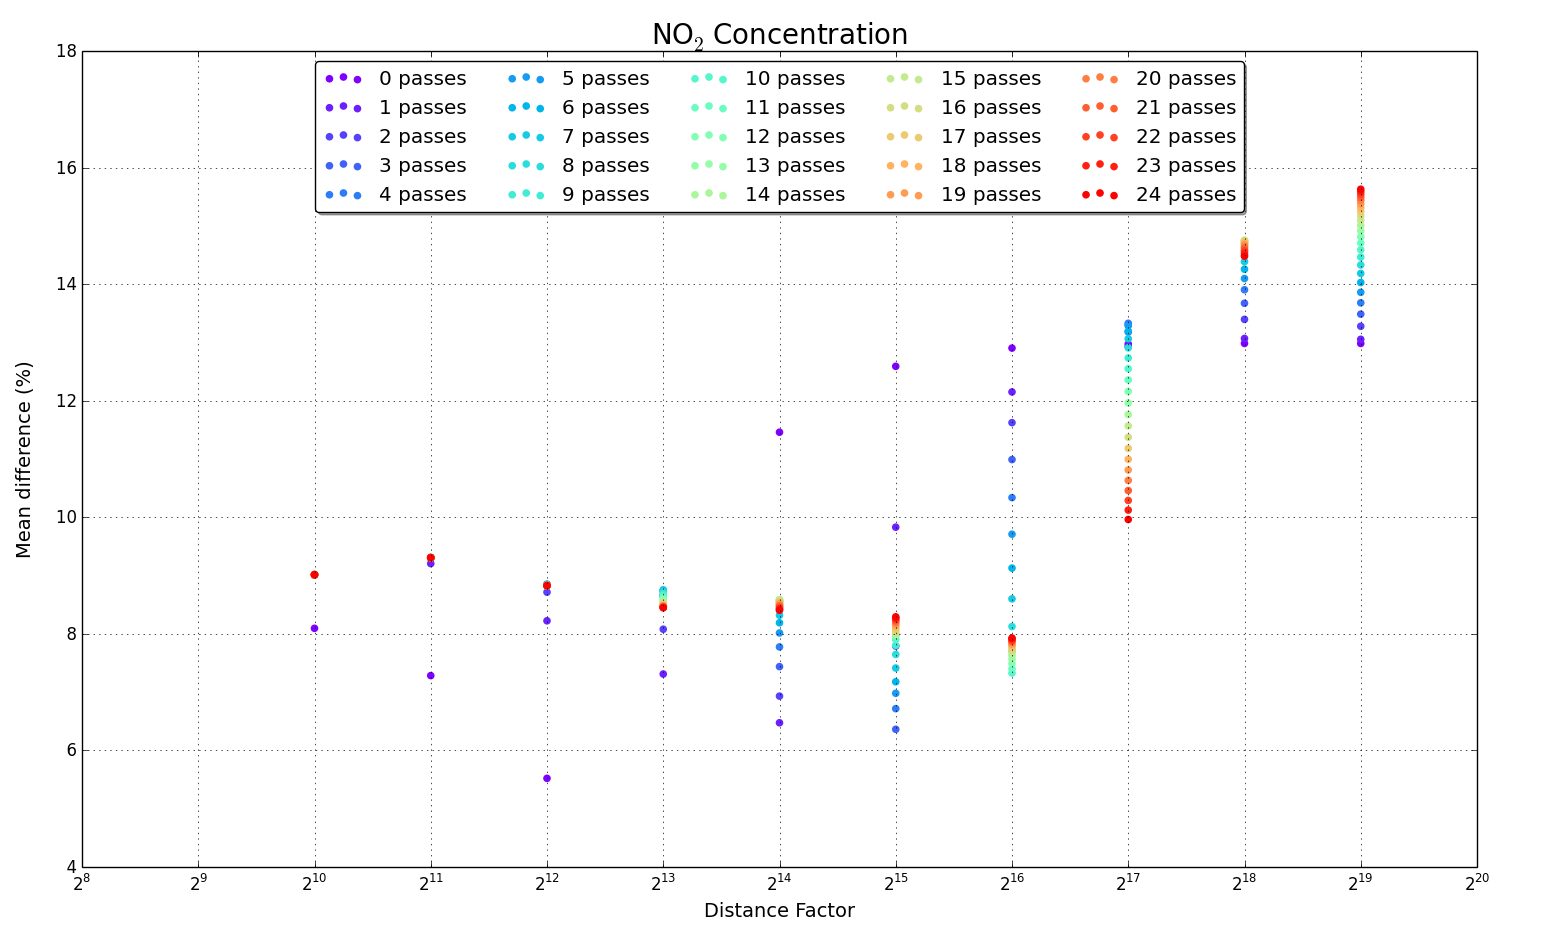
\includegraphics[width=\linewidth]{./images/Barnes_Distance_Factor_NO2.png}
                    \caption{Differences when applied to the $NO_{2}$ data in the Edinburgh data set.}
                    \label{fig:barnes_distance_factor_results_NO2}
                \end{subfigure}
                \begin{subfigure}{\textwidth}
                    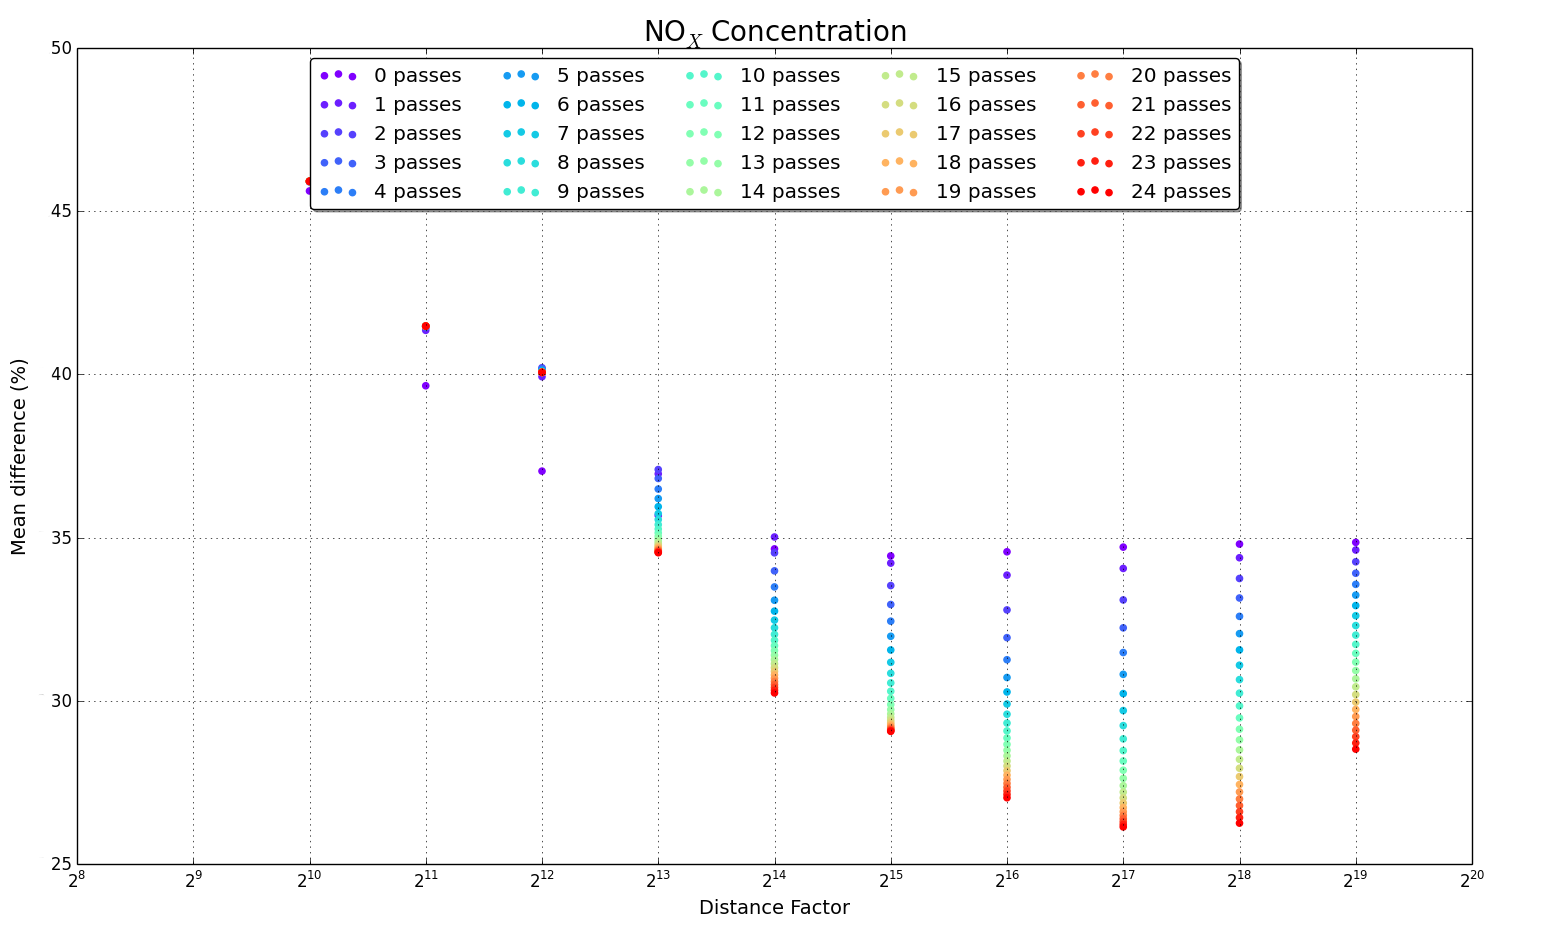
\includegraphics[width=\linewidth]{./images/Barnes_Distance_Factor_NOx.png}
                    \caption{Differences when applied to the $NO_{X}$ data in the Edinburgh data set.}
                    \label{fig:barnes_distance_factor_results_NOx}
                \end{subfigure}
                \caption{The difference between successive error correcting passes in Barnes interpolation when applied to the $NO_{2}$ and $NO_{X}$ data from the Edinburgh data set.}
                \label{fig:barnes_distance_factor_results_NO2_NOx}
            \end{figure}


        	The pollutants $NO$ and $NO_{X}$ appear to have the same tipping point in the distance factor, which is $2^{17}$. $NO_{2}$ is half of that distance at $2^{16}$. The graph also has a very different distribution, but this is not unexpected.

        	With the information of the distance factors, that is to say for $NO$, $NO_{2}$ and $NO_{X}$ the distance factors are $2^{17}$,$2^{16}$ and $2^{17}$ respectively, we must run the tests. The results of these tests are seen in table~\ref{tab:barnes_results}.

        	\begin{table}
				\centering
	    		\begin{tabular}{|c|c|c|}
	    			\hline
					Pollutant & Mean Difference (\%) & Distance Factor \\ \hline
					$NO$ & 15.73 & $2^{17}$\\
					$NO_{2}$ & 4.27 & $2^{16}$ \\
					$NO_{X}$ & 10.33 & $2^{17}$ \\
					\hline
				\end{tabular}
				\caption{The mean results of natural neighbour interpolation.}
				\label{tab:barnes_results}
			\end{table} 

		\subsection{OpenSense Data Set}\label{prediction_evaluation_results_opensense_data_set}

			As mentioned previously, the OpenSense data set arrived much later and was unable to be included in the initial tests. When the data set was received some initial analysis was run and the data set was shown to be inadequate for these purposes. In order to have a reasonable coverage of the city of Zurich, the temporal window was set to somewhere between 30 and 40 minutes depending on where we sliced the data set. Unfortunately this yielded results like those in figure~\ref{fig:opensense_bad_data}. We can see in this figure that we do not have smooth changes in ozone concentration along routes, instead the numbers appear to vary randomly. In small areas, such as the top left, we see data which is similar to what we would expect to see, which is small changes producing a smooth gradient. Unfortunately the majority of the data does not confirm to this expectation. Interpolation on this data set would, and indeed does, yield unpredictable results due to interpolation algorithms making the assumption that the discrete data points are part of a continuous data set, which this data does not seem to be. 

			\centerimage{0.7\textwidth}{./images/OpenSense_Ozone_Bad.png}{An example of the random nature of the OpenSense data set.}{fig:opensense_bad_data}

			However, the interpolation algorithms were applied to the data set in order to generate results. These results are shown in table~\ref{tab:opensense_interpolation_results}.

			\begin{table}
				\centering
	    		\begin{tabular}{|c|c|}
	    			\hline
					Algorithm & Mean Difference (\%) \\ \hline
					Barnes & 21.77\% \\
					Nearest Neighbour & 22.57\% \\
					IDW & 22.57\% \\
					Bicubic & 22.66\% \\
					Blurry Neighbour & 22.96\% \\
					Bilinear & 23.33\% \\
					Natural Neighbour & 24.44\% \\
					\hline
				\end{tabular}
				\caption{The results of the various interpolation algorithms on the OpenSense data set.}
				\label{tab:opensense_interpolation_results}
			\end{table} 

			These results immediate show that while the results are in the approximate range of the Edinburgh data set results, the ordering is different. From this our greatest performance, with the lowest deviation from the actual values, is the Barnes interpolation algorithm, followed by nearest neighbour, IDW, bicubic, blurry neighbour, bilinear and finally natural neighbour. 

			In terms of the blurry neighbour algorithm, we get our best results when sigma is equal to 1. The only better performance is when sigma is equal to 0, which is the same algorithm as nearest neighbour. As such we can immediately discount this algorithm. With respect to the IDW algorithm, the performance improved as the power parameter tended towards infinity. As discussed previously, this also approximates the nearest neighbour algorithm, and can therefore also discount IDW.

			One of the possible ways of breaking this analysis down is to split the mean results of both static stations into their two separate results. These are the differences for each of the measurement stations. The results of this are shown in table~\ref{tab:opensense_interpolation_split}.

			\begin{table}
				\centering
	    		\begin{tabular}{|c|c|c|}
	    			\hline
					Algorithm & Station 1 (\%) & Station 2 (\%) \\ \hline
					Nearest Neighbour & 41.48 & 3.66\% \\
					Barnes & 41.49 & 2.05\% \\
					Bicubic & 42.42 & 2.90\% \\
					Bilinear & 42.64 & 4.02\% \\
					Natural Neighbour & 42.70 & 6.18\% \\
					\hline
				\end{tabular}
				\caption{The mean results of the various interpolation algorithms on the OpenSense data set.}
				\label{tab:opensense_interpolation_split}
			\end{table} 

			From these results, the ordering for each station slightly changes. For the first station, Barnes moves to second, and nearest neighbour is in first place, followed by bicubic, bilinear and natural neighbour. With respect to the second station, Barnes is the clear winner, followed by bicubic, nearest neighbour, bilinear and then natural neighbour. The second stations results much more closely mimic the Edinburgh data set in terms of performance. 

			We can also see from this data set that we have a large discrepancy between the first stations results and the second stations results. The hypothesised reason for this is due to the time discrepancies. The temporal window for this data set is 36 minutes, however at station 2, our closest data point in figure~\ref{fig:opensense_bad_data} is only around 2-3 minutes old. At station 1, the difference is roughly 15 minutes. 

			This data set was originally planned on being used as it would be closest to a data set generated by buses moving around the city, however we have seen that the data set is inadequate for use with the algorithms presented above. This results in one of two possibilities. The first is that the data set is inconsistent as a result of the calibration process by the OpenSense group and that by understanding the nature of the data further, we could achieve better results with the simple algorithms above. However, the more likely conclusion is that when using cheap air quality sensors, and calibrating the results, we get a data set which is simply unsuitable for interpolation using simple algorithms. 

	\section{Conclusion}

		As has been stated multiple times in section~\ref{prediction_evaluation_results}, some results were unexpected and are attributed to a poor data set. The results in table~\ref{tab:all_results} are from the Edinburgh data set. 

		\begin{table}
			\centering
    		\begin{tabularx}{\linewidth}{|X|X|X|X|X|X|X|X|}
    			\hline
				Pollutant & Nearest Neighbour & Blurred Neighbour & IDW & Bilinear & Bicubic & Natural Neighbour & Barnes \\ \hline
				$NO$ & 23.87\% & 24.52\% & 24.98\% & 29.37\% & 18.38\% & 25.37\% & 15.73\% \\
				$NO_{2}$ & 3.75\% & 13.05\% & 7.59\% & 5.08\% & 4.10\% & 5.89\% & 4.27\% \\
				$NO_{X}$ & 13.49\% & 18.99\% & 18.98\% & 18.62\% & 11.22\% & 16.84\% & 10.33\% \\
				\hline
			\end{tabularx}
			\caption{The mean results of various interpolation method.}
			\label{tab:all_results}
		\end{table}

		

		\begin{table}
			\centering
    		\begin{tabularx}{\linewidth}{|X|X|X|X|X|X|X|X|}
    			\hline
				Pollutant & Nearest Neighbour & Blurred Neighbour & IDW & Bilinear & Bicubic & Natural Neighbour & Barnes \\ \hline
				$NO$ & 0.14714 & 0.15113 & 0.15398 & 0.18105 & 0.11328 & 0.15642 & 0.09700 \\
				$NO_{2}$ & 0.08571 & 0.29845 & 0.17360 & 0.11613 & 0.09370 & 0.13476 & 0.09764\\
				$NO_{X}$ & 0.12434 & 0.17507 & 0.17504 & 0.17164 & 0.10345 & 0.15525 & 0.09521 \\ \hline
				Mean & 0.11906 & 0.20822 & 0.16754 & 0.15627 & 0.10348 & 0.14881 & 0.09662 \\
				\hline
			\end{tabularx}
			\caption{The relative performance of the interpolation methods.}
			\label{tab:all_ratio_results}
		\end{table}

		\centerimagewideanywhere{./images/Algorithm_Performance_Ratio.png}{The relative performance of the interpolation methods.}{fig:all_ratio_results}

		Alone this data provides very little information, as we have no way of comparing algorithms should one be better at a particular pollutant than the other. In order show this, we have normalised the results across the pollutants. Table~\ref{tab:all_ratio_results} and figure~\ref{fig:all_ratio_results} show these results. Using these normalised metrics we can see that our best performing algorithm is the Barnes algorithm. This result is followed closely by the bicubic algorithm and then nearest neighbour. Unfortunately these results immediately betray one of the earlier points of interest. It was hypothesised that if an algorithm approximated another, but had tunable parameters, then we would see results which were better than the original algorithm, when tuned for the specific situation. The ranking of the bicubic algorithm above the blurry neighbour algorithm shows that this hypothesis is incorrect, at least for this data set. 

		With the Edinburgh data set, due to the low number of data points, we cannot confirm that the comparisons of these algorithms for pollutant data is correct with any high degree of certainty. We can however state that it is likely that Barnes interpolation would perform the best given that research indicated its accuracy in these applications. Barnes interpolation is unfortunately also the slowest method of interpolation tested. As such it may be wise to use a slightly faster algorithm in a real world approach. A further, better, approach may be to use different algorithms for different pollutants.

		We have shown which algorithms perform better relative to the others, however the question of whether these results are good enough to be used remains open. With Barnes giving us an accuracy of between 4\% and 16\%, these results must be respected given that they come from on of the simpler interpolation algorithm which exist. A variation of 16\% means that we could see concentrations of $NO$ varying by up to 70$\mu gm^-3$, $NO_{2}$ by 20-25$\mu gm^-3$ and $NO_{X}$ by 90-100$\mu gm^-3$, based on the data set used. These variations could be the difference between safe levels and those hazardous to ones health. As such, these simple interpolation algorithms can yield approximate information about pollutant levels in unknown locations, however, they are unlikely to be of use in the field of air quality monitoring. 
